\section{Werkzeuge}
Grundsätzlich standen uns zwei Werkzeuge zur Modellierung von Geschäftsprozessen zur Verfügung, die KIE Workbench als Webanwendung und der BPMN 2.0 Modeler als Eclipse-Plugin.
\subsection{KIE Workbench}
Die KIE Workbench tritt als Allrounder auf. Von eigenen Gestaltungsoberflächen für Prozesse und Formulare über Projektverwaltung und Deployment in eine Runtime bis hin zur Benutzerverwaltung erfüllt sie unser gesamtes Anforderungsspektrum. Die Workbench vermittelte den Eindruck äußerst realitätsnah und in der freien Wirtschaft einsetzbar zu sein. Entsprechend optimistisch waren wir unser Projekt in dieser Umgebung umzusetzen.

Leider mussten wir schon nach wenigen Stunden diverse Grenzen und Nachteile der Workbench entdecken. Neben einer gewissen Unübersichtlichkeit aufgrund des Umfang der Workbench, gab es keine Möglichkeit den entwickelten Prozess zu debuggen. Darüber hinaus ist die Webanwendung nur auf Monitoren mit hoher Auflösung komfortabel einsetzbar, was in unserem Fall erhebliche Probleme mit der Übersichtlichkeit und Bedienbarkeit des Prozessdesigners bedeutete. Die Abbildung \ref{fig:KieWorkbench} zeigt die KIE Workbench, wie wir sie zu nutzen versuchten. Des Weiteren war die Arbeitsweise des Zusammenklickens ohne weiterführende Kontrollmöglichkeiten für uns als Softwareentwickler etwas befremdlich. Letztendliches Ausschlusskriterium war allerdings, dass der Designer nicht ausgereift ist und mehrmals das BPMN zugrunde liegende XML-Dokument zerstörte und invalides und somit unbrauchbares XML zurückließ. 

Aufgrund der aufgezählten Hindernisse haben wir uns für die Alternative, den BPMN 2.0 Modeler im Eclipse, entschieden.

\begin{figure}[H]
\centering
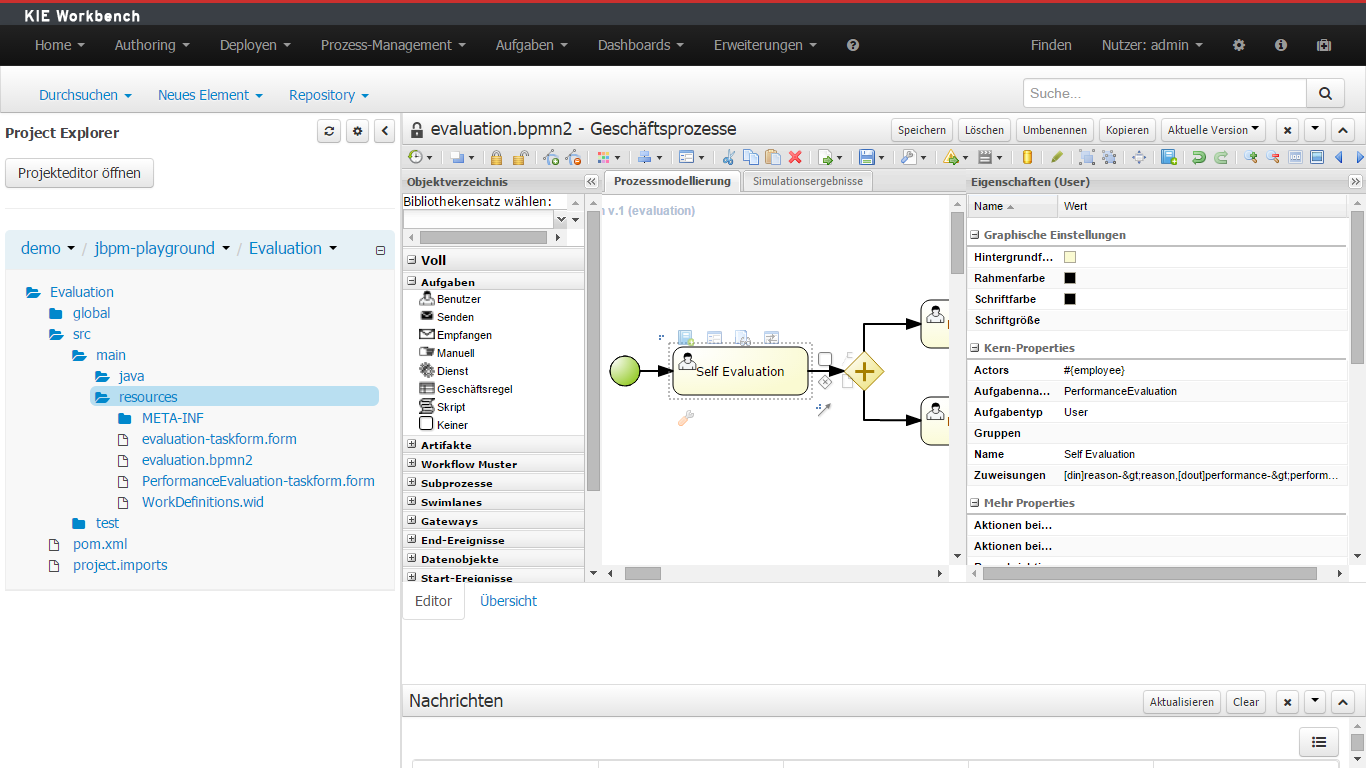
\includegraphics[width=0.9\linewidth]{../Bilder/KieWorkbench}
\caption{KIE Workbench Prozesseditor}
\label{fig:KieWorkbench}
\end{figure}

\subsection{Eclipse BPMN 2.0 Modeler}
Der BPMN 2.0 Modeler ist ein Plugin für die Eclipse Entwicklungsumgebung. Das Plugin ermöglicht eine relativ intuitive und komfortable Gestaltung von Geschäftsprozessen. In Kombination mit der Entwicklungsumgebung und der Implementierung eigener Workitemhandler in Java und Instanziierung einer KIE Runtime wird Debuggen ermöglicht und uns als Entwickler mehr Kontrolle über die Geschehnisse gegeben. Aufgrund der Zuverlässigkeit des Designers und trotz der Mehraufwände besonders durch die Implementierung einer grafischen Benutzerschnittstelle, war die Wahl des BPMN Modeler und die Umsetzung in Eclipse die bessere Entscheidung. 